\chapter{Antecedentes}
\label{ch:background}
En el presente Cap\'itulo se exponen conceptos cruciales para la comprensi\'on y desarrollo de este trabajo. Se describen en particular los objetos de inter\'es que estimularon el desarrollo del survey HiTS: las supernovas de tipo II y el evento de shock-breakout asociado a \'estas y una breve descripci\'on de los datos obtenidos por este proyecto durante el a\~no 2015. De la misma forma, se describe la base matem\'atica en la que se basan las diferentes versiones del filtro de Kalman implementadas en el software original, es decir, los filtros de Kalman \textit{b\'asico} y de \textit{m\'axima correntrop\'ia} as\'i como una nueva versi\'on del m\'etodo conocida como \textit{unscented} que permitir\'ia la introducci\'on de modelos no lineales en el proceso de filtrado.  

\section{Supernova tipo II}\label{sec:sn}
Una supernova de tipo II corresponde a un evento estelar con el que finaliza la vida de una estrella masiva (aquellas que en su proceso de formaci\'on poseen una masa superior a 10 masas solares \footnote{$M_{\odot} = (1.98847 \pm 0.00007) \times 10^{30}$ Kg}). Al no contar con combustible necesario para llevar a cabo reacciones nucleares que puedan contrarrestar su propia gravedad (su n\'ucleo ya no puede formar elementos m\'as pesados que el hierro o el n\'iquel, los cuales caen al n\'ucleo de la estrella por su propio peso. Ver Figura \ref{fig:f0}.), y si la presi\'on degenerada\footnote{presi\'on que viene del principio de exclusi\'on de Pauli} de los electrones del plasma de la estrella no es suficiente para soportar este peso, la estrella se contrae abruptamente incrementando la temperatura de su centro a, aproximadamente, $10^{10}$ K.
\bigskip

\begin{figure}[h!]
\centering
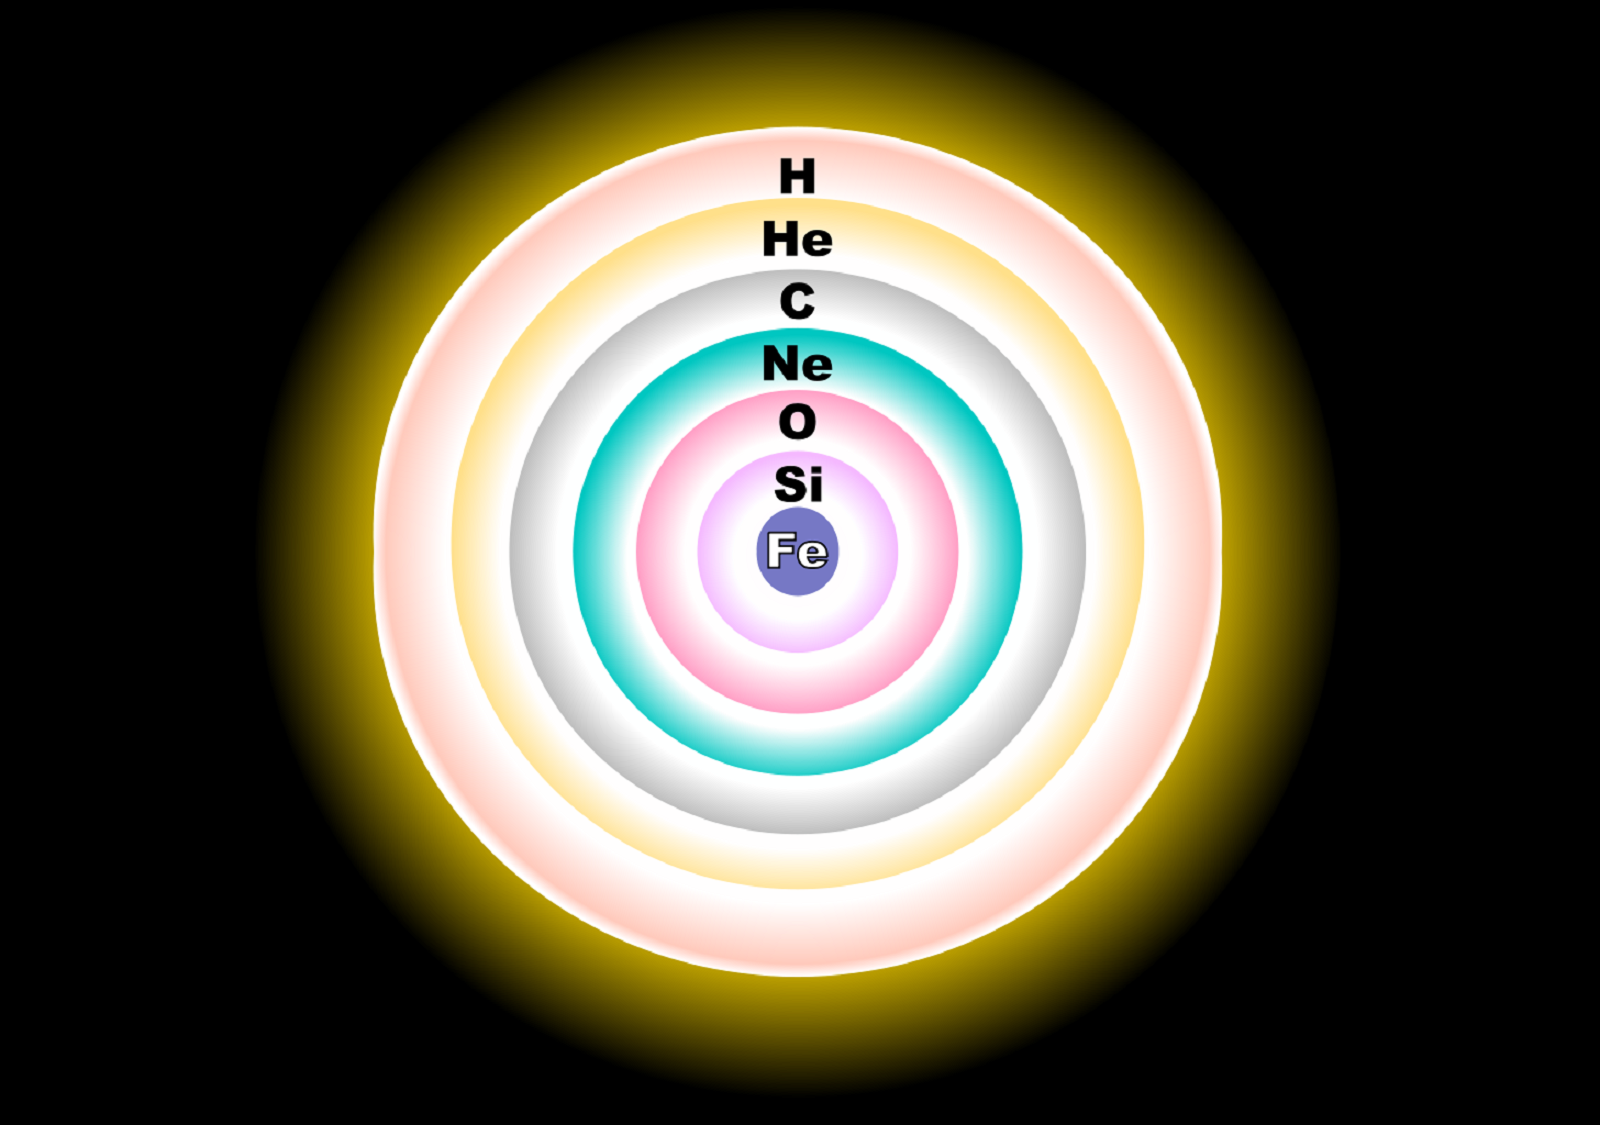
\includegraphics[scale=.25]{images/sncore}
\caption{Esquema no a escala de la estructura de una estrella masiva previo a su explosi\'on como supernova. Los elementos m\'as pesados se alojan en el centro, mientras que  los m\'as livianos, como el hidr\'ogeno o el helio lo hacen en la capa m\'as externa. \textit{Imagen publicada por R. J. Hall en WikiMedia Commons, 15 de agosto de 2007.}}
\label{fig:f0}
\end{figure}


Debido al aumento de temperatura, los electrones del n\'ucleo adquieren energ\'ia cin\'etica suficiente para escapar, desapareciendo as\'i la presi\'on que ejerc\'ian hacia el exterior. Finalmente el n\'ucleo colapsa liberando energ\'ia gravitacional y con ella las capas m\'as externas de la estrella son expulsadas en una gran explosi\'on. Este fen\'omeno se denomina \textit{supernova} e implica un aumento repentino del brillo de una estrella, incrementando su brillo en un factor de $10^8$ veces, pudiendo incluso ser m\'as brillante que la galaxia que la alberga.
\bigskip

En general la variaci\'on de la luminosidad de una supernova corresponde a una curva que crece r\'apidamente los primeros d\'ias (u horas), alcanzando un m\'aximo, para luego decaer. Cabe destacar que existen otros tipos de supernova, c\'omo las de tipo Ia que corresponden a otro fen\'omeno en donde participa una clase de estrella denominada enana blanca junto a otra estrella de cualquier otro tipo. La primera, al poseer una gravedad tan alta en su superficie es capaz de tomar material de su compa\~nera con lo que al superar las 1.44 $M_{\odot}$ se desencadenar\'ia la explosi\'on de una supernova. 
\bigskip

Las supernovas de tipo Ia presentan un decaimiento casi continuo una vez alcanzado el m\'aximo, mientras que las de tipo II presentan dos ca\'idas: una inmediatamente despu\'es de su m\'aximo y otra una vez finalizado un per\'iodo de decaimiento suavizado (ver Figura \ref{fig:f1}). Otra forma de diferenciarlas es la presencia de trazas de hidr\'ogeno en los espectros de \'estas: las supernovas de tipo Ia pr\'acticamente no presentan hidr\'ogeno (l\'ineas de absorci\'on distintivas) a diferencia de las de tipo II.\bigskip

\begin{figure}[h!]
\centering
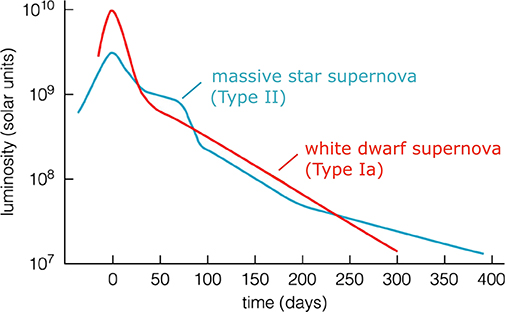
\includegraphics[scale=.8]{images/clear}
\caption{Curvas t\'ipicas de supernovas Ia (enana blanca) y II (estrella masiva). \textit{\textcopyright 2004 Pearson Education Inc., publishing as Addison-Wesley The Bizarre Stellar Graveyard.}}
\label{fig:f1}
\end{figure}


\section{High Cadence Transient Survey: HiTS}

El High Cadence Transient Survey\cite{hits} (desde ahora, HiTS) es un survey cuyo objetivo principal es detectar y seguir fen\'omenos transitorios estelares en escalas de tiempo que van desde horas a d\'ias, con especial atenci\'on a fases tempranas de explosiones de supernovas (primeras horas). Sin embargo, el objetivo original de HiTS corresponde a la detecci\'on de un fen\'omeno llamado \textit{shock breakout} (SBO), un fen\'omeno que ocurre inmediatamente despu\'es del colapso del n\'ucleo de una estrella roja supergigante (una de las posibles etapas finales de una estrella masiva antes de \textit{explotar} en supernova II). Ver Figura \ref{fig:f2}\footnote{$L_{\odot}= 3.828 \times 10^{26}$ W}.

%\ref{fig:f2}\footnote{\url{https://www.nasa.gov/feature/ames/Kepler/caught-for-the-first-time-the-early-flash-of-an-exploding-star}}


\begin{figure}[h!]
\centering
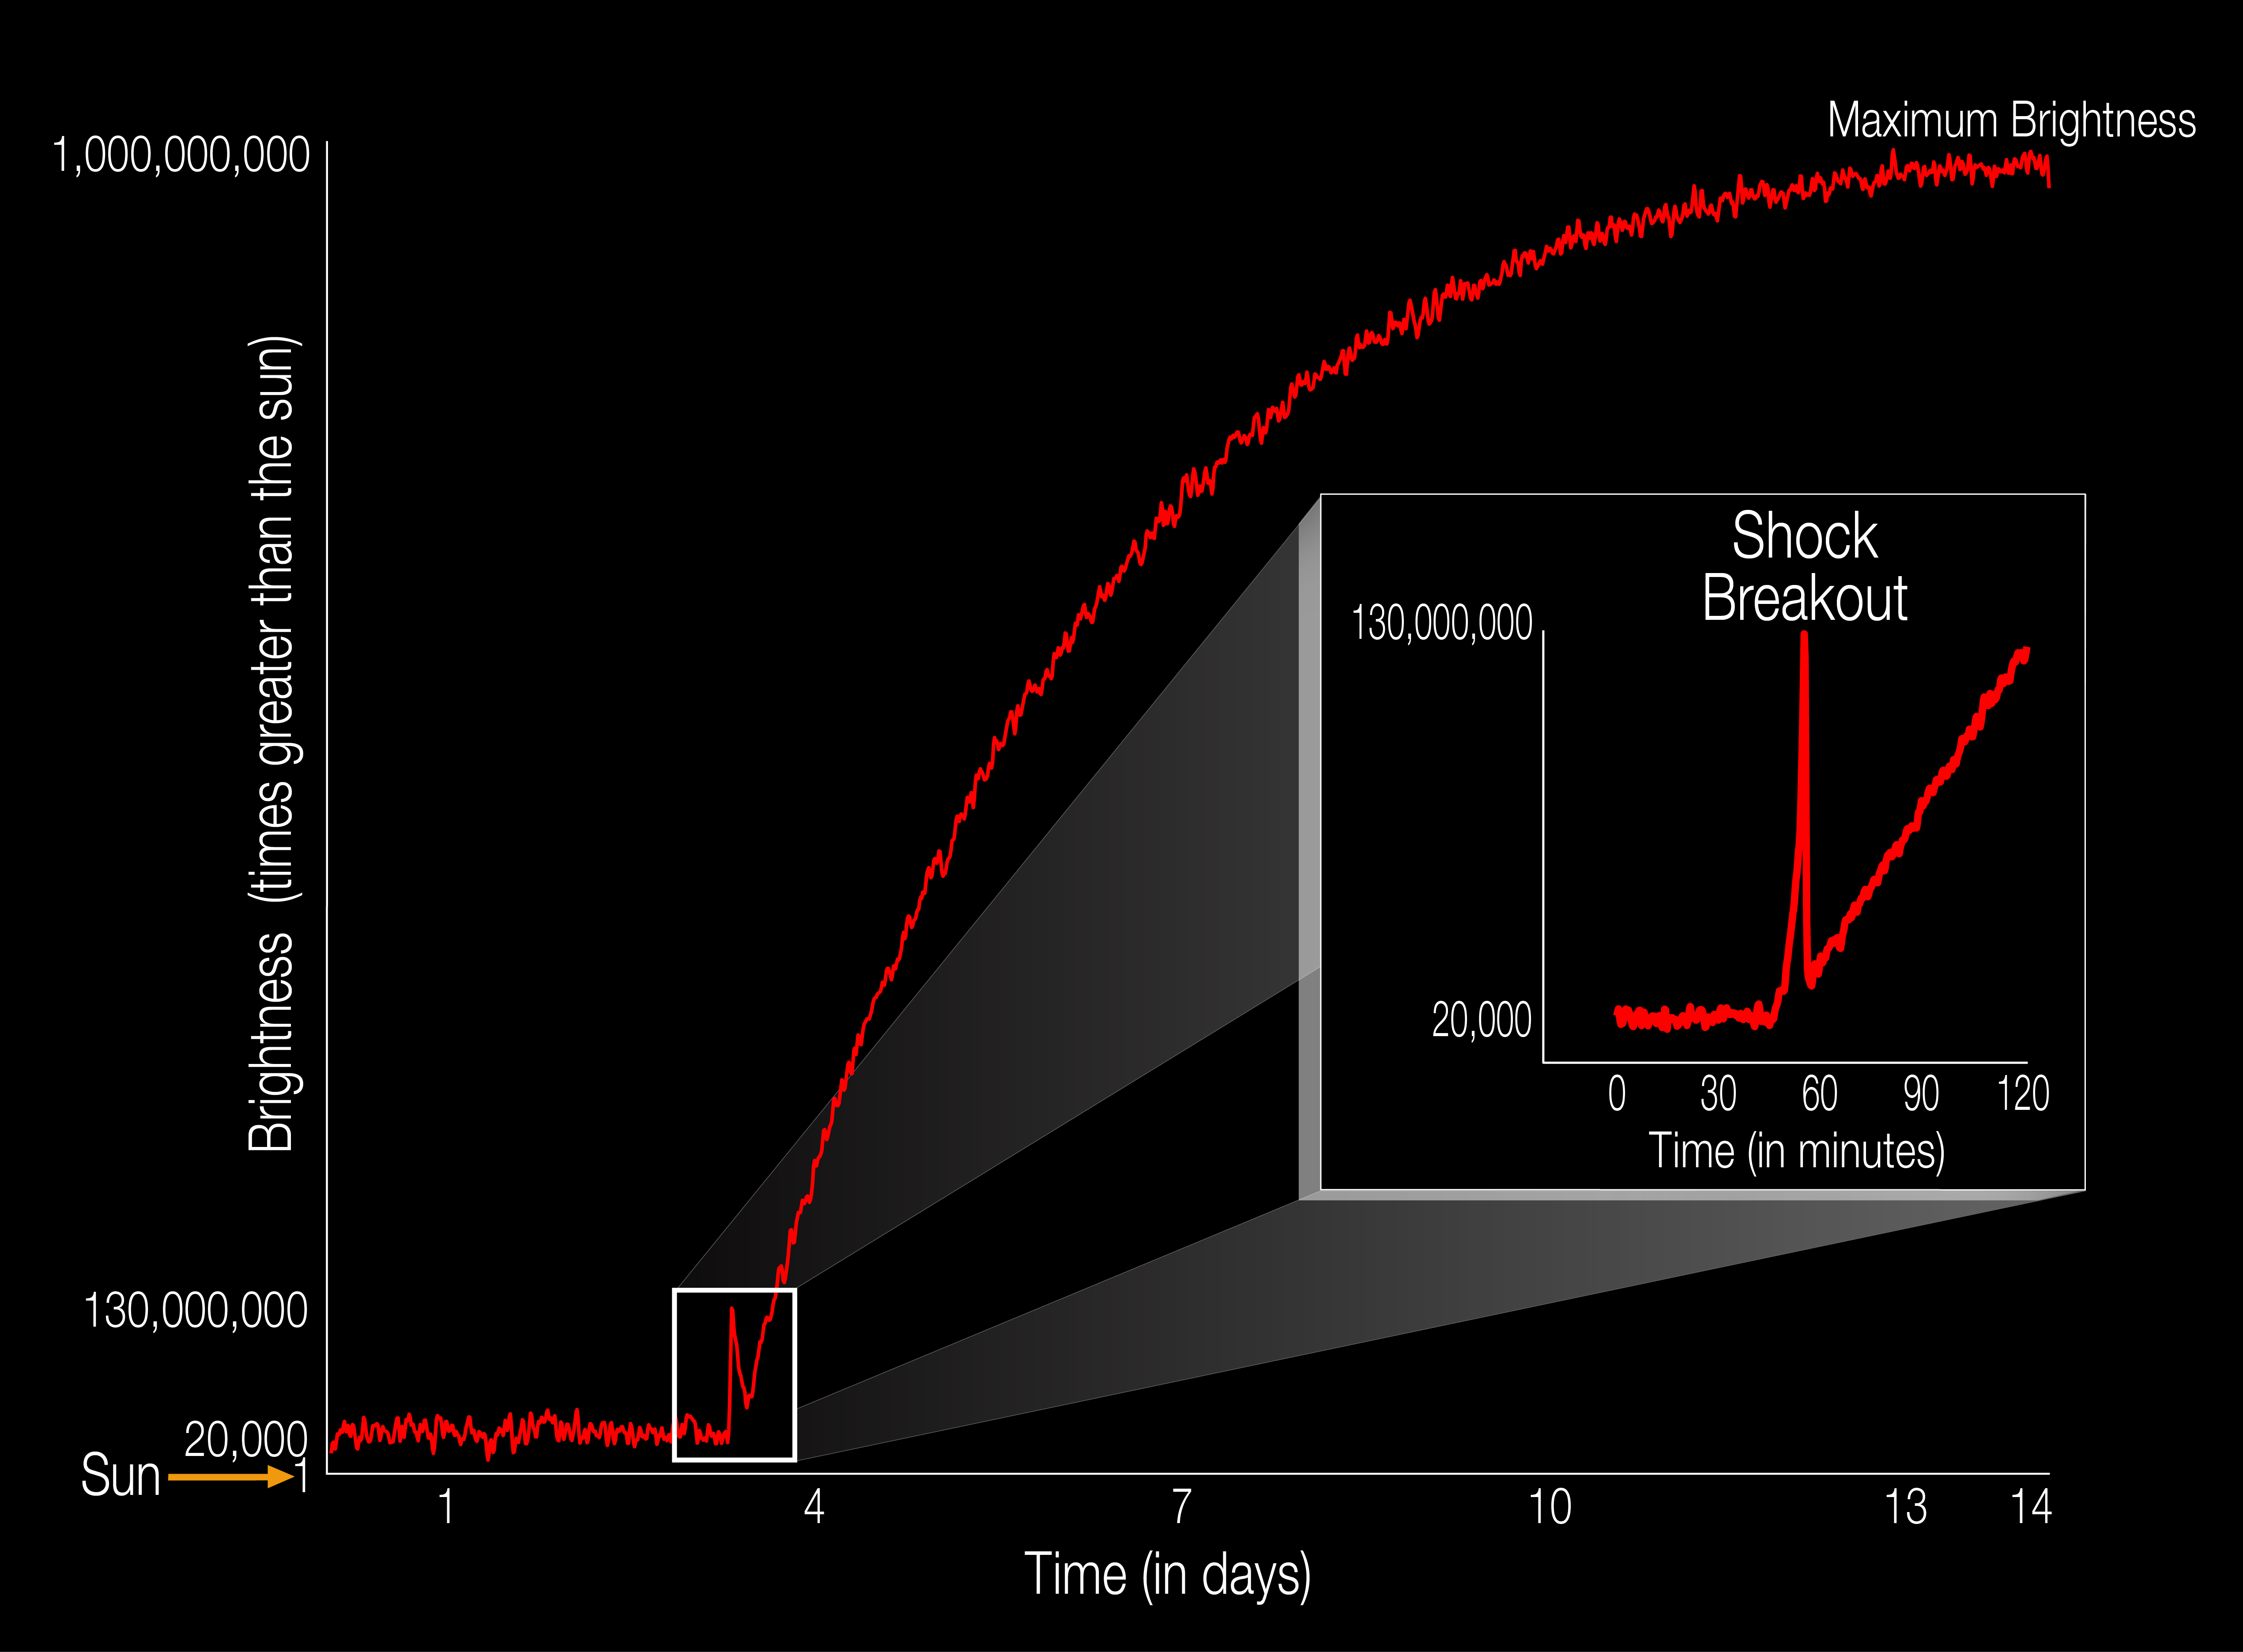
\includegraphics[scale=.25]{images/breakout}
\caption{Diagrama que ilustra la evoluci\'on del brillo de una supernova en t\'erminos de luminosidad solar ($L_{\odot}$) durante d\'ias. Se resalta el fen\'omeno de \textit{shock-breakout} apenas comienza el incremento de la luminosidad de la supernova. Esta imagen fue publicada en la p\'agina de la NASA destacando la primera vez que un evento como este es \textit{capturado} en la banda visible (por el telescopio espacial Kepler). \textit{NASA Ames/W. Stenzel, 2016.}}
\label{fig:f2}
\end{figure}

HiTS utiliza la Dark Energy Camera (DECam, ver Figura \ref{fig:f3}) para la obtenci\'on de sus im\'agenes. Esta c\'amara se encuentra montada en el Telescopio Blanco del Observatorio de Cerro Tololo (CTIO) en la regi\'on de Coquimbo, Chile. Esta c\'amara posee 62 detectores CCD de $2048 \times 4096$ p\'ixeles para la obtenci\'on de im\'agenes cient\'ificas y otros 12 para la gu\'ia, alineamiento y enfoque (ver Figuras \ref{fig:f3} y \ref{fig:f4} d\'onde se muestra disposici\'on de las c\'amaras CCD en el telescopio). 
\bigskip

\begin{figure}[h!]
\centering
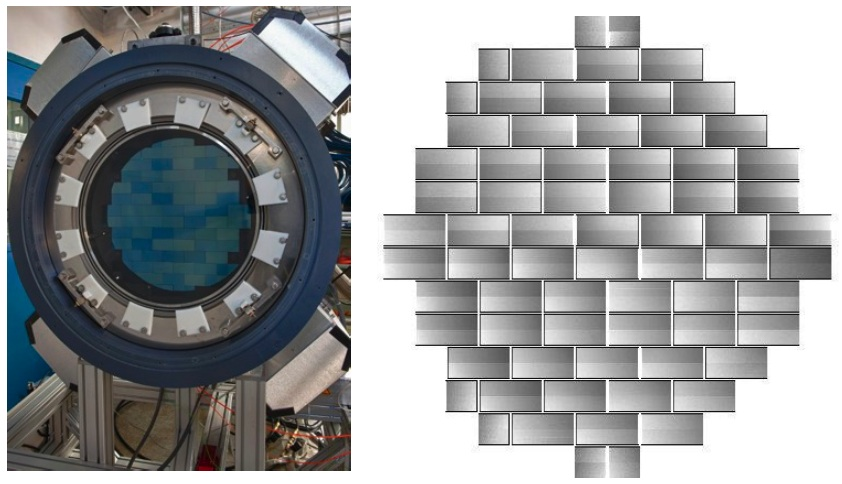
\includegraphics[scale=.5]{images/CCDs.jpg}
\caption{A la izquierda, estructura de la c\'amara DECam poblada con 62 chips CCDs. A la derecha, imagen \textit{flat field} desde DECam. \textit{Im\'agenes tomadas desde la p\'agina del Dark Energy Survey (\url{www.darkenergysurvey.org/the-des-project/instrument/the-camera}).}}
\label{fig:f3}
\end{figure}

Durante el proyecto HiTS se realizaron tres campa\~nas de observaci\'on en los a\~nos 2013, 2014 y 2015 durante el primer semestre de cada a\~no. Se escogieron 40 campos y 4 \'epocas por noche (tambi\'en por campo) para observaciones realizadas en el 2013 y el 2014. Para la campa\~na del a\~no 2015 se escogieron 50 campos. En estas campa\~nas se obtuvieron m\'as de 120 candidatos a supernova. Sin embargo, no se logr\'o encontrar en estas rastros de SBO, evento que comprendi\'o uno de los principales objetivos de HiTS. La distribuci\'on de los campos observados, por a\~no, se describe en la Figura \ref{fig:fields}. 

\begin{figure}[h!]
\centering
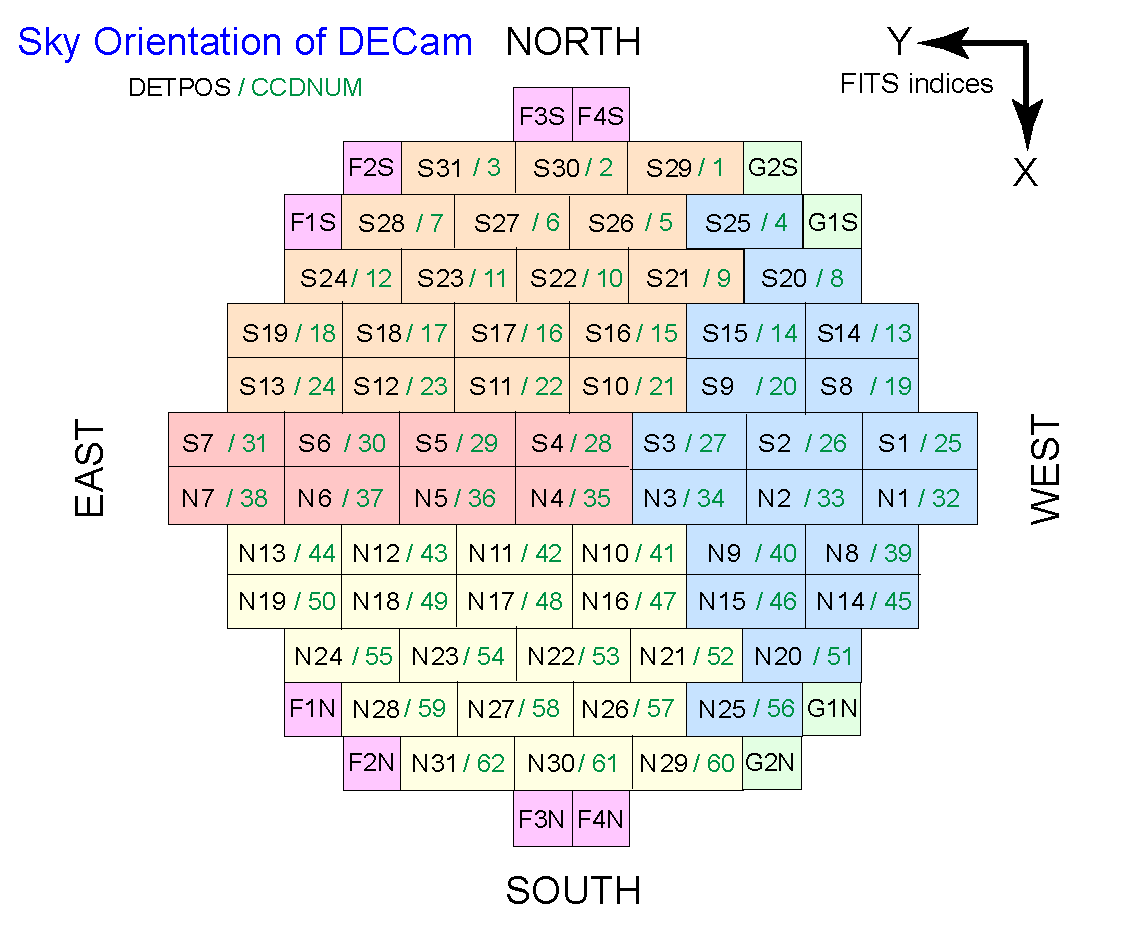
\includegraphics[scale=.75]{images/decam}
\caption{Orientaciones sobre el cielo y la huella espacial del arreglo de detectores en el plano focal. Se destacan los CCD cuya etiqueta comienzan con S o N, ya que estos corresponden a los detectores encargados de obtener las im\'agenes cient\'ificas. El etiquetado de estas componentes puede ser enga\~noso debido a que las iniciales de norte (North) y sur (South) est\'an invertidas en relaci\'on a la orientaci\'on del cielo. \textit{Imagen publicada en el sitio del CTIO (\url{http://www.ctio.noao.edu/noao/node/2250})}.}
\label{fig:f4}
\end{figure}

\begin{figure}
\centering
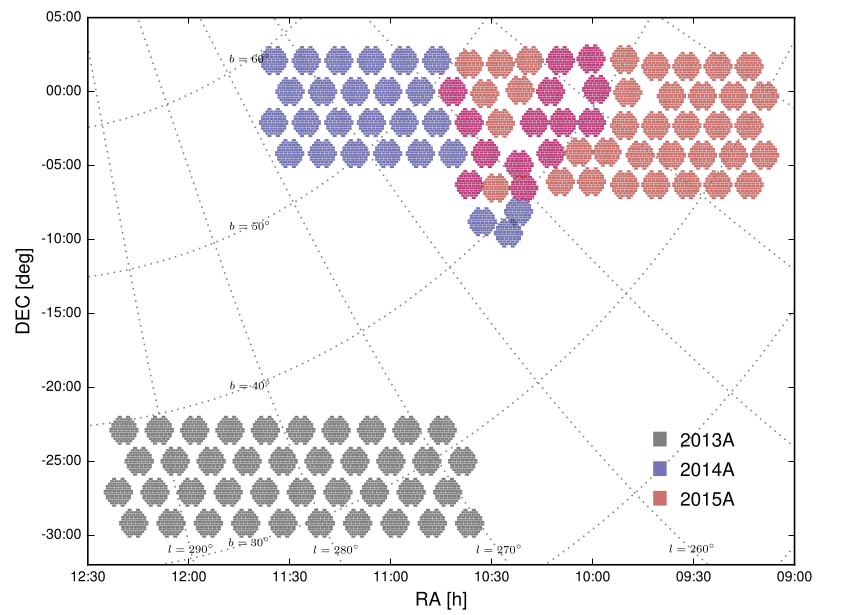
\includegraphics[scale=.5]{images/fields}
\caption{Distribuci\'on espacial de los campos observados durante los primeros semestres de los a\~nos 2013 (gris), 2014 (azul) y 2015 (naranjo). En tono rojo, los mismos campos del a\~no 2015 y 2014 (superposici\'on). \textit{F. F\"orster et al., 2015. HiTS real-time supernova detections.}}
\label{fig:fields}
\end{figure}

\subsection{Datos obtenidos durante el a\~no 2015}\label{ssec:data}
Como se mencion\'o anteriormente, la campa\~na del a\~no 2015 tuvo lugar el primer semestre de ese a\~no. El per\'iodo en que se llev\'o a cabo fue durante los meses de febrero y marzo; espec\'ificamente entre los d\'ias 17 de febrero y 14 de marzo.
\bigskip

El per\'iodo comprendido por los d\'ias 17 a 22 de febrero fue el de mayor latencia, obteni\'endose hasta cinco \'epocas (observaciones) por noche por cada campo. Posteriormente la toma de observaciones cesa y se reanuda a partir del 25 de febrero con una latencia de a lo m\'as tres \'epocas por noche y campo, con interrupciones de hasta nueve d\'ias finalizando el 14 de marzo (ver Figura \ref{fig:cadencia}). 

\begin{figure}
\centering
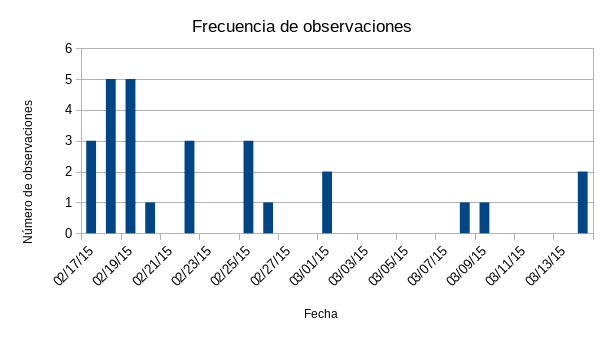
\includegraphics[scale=1.0]{images/cadencia}
\caption{Frecuencia de las observaciones realizadas en el survey de HiTS durante el semestre del a\~no 2015.}
\label{fig:cadencia}
\end{figure}

\section{El filtro de Kalman}
La evoluci\'on determin\'istica de un sistema f\'isico en el tiempo es conocida si el estado del sistema es medido con absoluta precisi\'on en cada instante de tiempo (i.e., en un entorno donde es posible despreciar fen\'omenos cu\'anticos). Sin embargo toda medici\'on est\'a sujeta a incertezas finitas. Para sistemas que son observados en intervalos prolongados de tiempo, se prevee que las diferencias entre los estados estimados y los medidos se incrementen con el tiempo. Para la obtenci\'on de predicciones lo m\'as confiables posible se requiere que el sistema sea regularmente monitoreado y sus estados estimados puedan ser considerados confiables en un lapso de tiempo apropiado. 
\bigskip

Los filtros de Kalman son m\'etodos que proveen un compromiso (o trade-off) entre los valores esperados del estado actual de un sistema y las mediciones que proporcionan informaci\'on de su estado real. La aplicaci\'on de un filtro de Kalman est\'a pensada como un proceso de dos fases:
\begin{enumerate}
\item \textbf{Fase predictiva:} Una \textit{apuesta} del estado actual del sistema que se basa en un modelo f\'isico (determin\'istico). Esta cantidad se denomina usualmente como estado estimado \textit{a priori}. 
\item \textbf{Fase correctiva:} La estimaci\'on del estado \textit{a priori} es corregida con una medida real del sistema con la que se obtiene la predicci\'on; con ella se procede a calcular una cantidad conocida como \textit{ganancia de Kalman} con la que se estima una \textit{aproximaci\'on a posteriori} del sistema, evaluando que tan lejos estuvo nuestra aproximaci\'on \textit{a priori}. 
\end{enumerate}
\bigskip

T\'ipicamente estas fases de predicci\'on y correcci\'on se van alternando mientras se estudia el comportamiento f\'isico de alg\'un sistema. En particular, esto filtros son bastante usados en procesos como el guiamiento de un m\'ovil, en sistemas de navegaci\'on y en an\'alisis de se\~nales; contextos en los cuales el monitoreo de estado de un sistema puede ser m\'as que relevante.
\bigskip

En las subsecciones siguientes se har\'a uso de la notaci\'on de sub\'indices $m|n$, en las estimaciones de estado y covarianzas, para explicitar el instante de tiempo al cual pertenecen:  $m$; y al instante de tiempo de donde se extrae la informaci\'on: $n$. Se har\'a uso de la notaci\'on $k$ para referirse al estado actual y de $k-1$ y $k+1$ para indicar los instantes anterior y pr\'oximo a $k$, respectivamente.
\bigskip

\begin{itemize}
\item $\hat{x}_{k-1|k-1}$: Estado estimado en el paso anterior ($k-1$) o estado inicial del modelo. Es un vector de largo $N$, donde $N$ es el n\'umero de variables de estado a estudiar.
\item $P_{k-1|k-1}$: Matriz de covarianza asociada al estado estimado en el paso anterior o matriz de covarianza inicial. Posee dimensi\'on $N\times N$.
\end{itemize}
\bigskip

Durante la fase predictiva se obtienen las cantidades detalladas a continuaci\'on:
 
\begin{itemize}
\item $\hat{x}_{k|k-1}$: Estado estimado \textit{a priori} (vector de dimensi\'on $N$). 
\item $P_{k|k-1}$: Matriz de covarianza \textit{a priori} (matriz de dimensi\'on $N\times N$ ).
\end{itemize}
\bigskip

Luego, en la fase de correcci\'on se recibe como entrada la medici\'on realizada en el tiempo $k$, $z_k$, y se calculan las siguientes cantidades:

\begin{itemize}
\item $\hat{z}_k$ : Combinaci\'on del estado estimado \textit{a priori}, $\hat{x}_{k|k-1}$ y la medici\'on real, $z_k$. Corresponde a la correcci\'on, propiamente tal.
\item $\tilde{z}_k$ : Diferencia entre la medici\'on real, $z_k$, y la correcci\'on $\hat{z}_k$.
\item $\hat{x}_{k|k}$ : Estado estimado \textit{a posteriori} o estado actualizado.
\item $P_{k|k}$ : Matriz de covarianza \textit{a posteriori} (actializada).
\end{itemize}
\bigskip
 
\begin{figure}
\centering
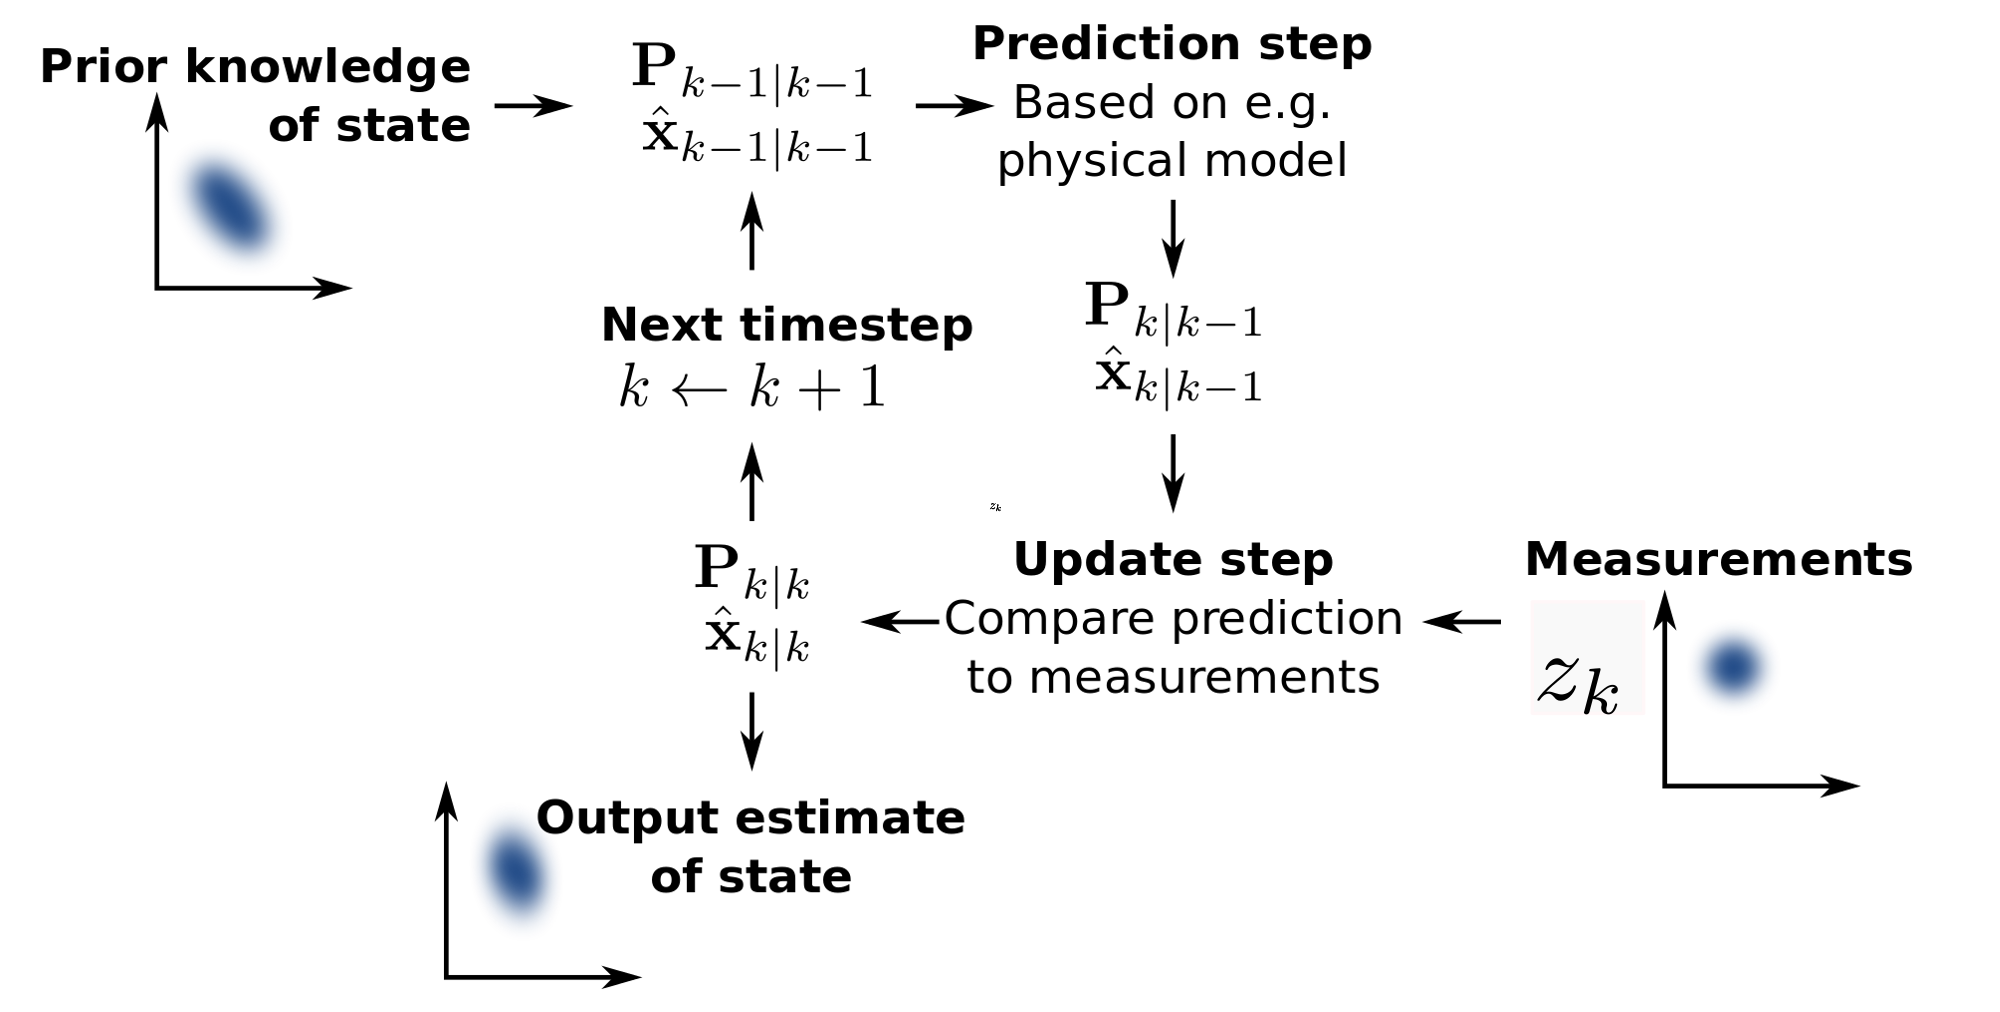
\includegraphics[scale=.2]{images/diag_kalman}
\caption{Diagrama del proceso de estimaci\'on de estados. El filtro de Kalman ``sigue la pista'' del estado f\'isico de un sistema, estim\'andolo paso a paso. El proceso comienza con la entrada de los valores $\hat{x}_{k-1|k-1}$ y $P_{k-1|k-1}$, determinados en el instante $k-1$. Para obtener la estimaci\'on del estado en el instante actual, $k$, se hace una predicci\'on a partir de la informaci\'on m\'as reciente (obtenida en $k-1$) y del modelo f\'isico escogido, obteni\'endose as\'i los valores de $\hat{x}_{k|k-1}$ y $P_{k|k-1}$. Luego durante la fase correcci\'on esta predicci\'on es corregida con la observaci\'on $z_k$ y con ello, se actualizan los valores del estado predicho y de la matriz de covarianza en $\hat{x}_{k|k}$ y $P_{k|k}$, respectivamente. Finalmente estas \'ultimas cantidades se transformar\'an en la entrada del algoritmo para el tiempo $k+1$. \textit{Imagen publicada por P. Aimonen en Wikimedia Commons, en noviembre de 2011.}}
\label{fig:diag}
\end{figure} 
 
El proceso de estimaci\'on (predicci\'on y correcci\'on) puede resumirse en el diagrama de la Figura ~\ref{fig:diag}. 
 
\subsection{Filtro de Kalman B\'asico}
El filtro de Kalman B\'asico \cite{kalman} asume un comportamiento de sistema lineal y que las mediciones y las predicciones siguen una distribuci\'on Gaussiana. 
\bigskip

A continuaci\'on se describen las componentes del desarrollo matem\'atico del filtro:

\begin{itemize}
\item \textbf{$F_k$:} Matriz de transici\'on de estado, de dimensiones $N\times N$.
\item \textbf{$H_k$:} Matriz de transformaci\'on de estado a medici\'on, $K\times N$ (K corresponde al n\'umero de variables de estado medidas en un instante $k$, y puede ser menor a $N$).
\item \textbf{$Q_k$:} Matriz de covarianza del ruido del proceso ($N\times N$).
\item \textbf{$R_k$:} Matriz de covarianza del ruido de las mediciones ($K\times K$).
\item \textbf{$B_k$:} Matriz de control de entrada (contiene alteraciones que se querr\'ian agregar al sistema de manera deliberada, por ejemplo, como la condici\'on de parada de un veh\'iculo en movimiento). Esta matriz es de dimensiones $N\times L$, donde $L$ es la dimensi\'on del vector de control de entrada $u_k$.
\item \textbf{$q_k$:} Corresponde al ruido del proceso modelado, en las variables de estado. Posee una distribuci\'on normal multivariada y centrada en cero, con una matriz de covarianza $Q_k$.
\end{itemize}
\bigskip


Con estas variables, podemos describir las ecuaciones que explican la evoluci\'on del proceso del algoritmo de Kalman b\'asico (un esquema de los c\'alculos involucrados en el proceso de estimaci\'on de estados se puede ver en la Figura \ref{fig:kfb}):
\begin{enumerate}
\item \textbf{Fase predictiva:}\\
Las ecuaciones de estimaci\'on de estado y matriz de covarianza \textit{a priori} son:
\begin{equation}
\hat{x}_{k|k-1} = F_k \hat{x}_{k-1|k-1} + B_k u_k,
\label{eq:eq1}
\end{equation}
\begin{equation}
P_{k|k-1} = F_{k}P_{k-1|k-1}F_k^{T} + Q_k. 
\label{eq:eq2}
\end{equation}
\item \textbf{Fase correctiva:}\\
El proceso de correcci\'on comienza con la determinaci\'on de las siguientes cantidades:
\begin{equation}
\hat{z}_k = H_{k} \hat{x}_{k|k-1},
\label{eq:eq3}
\end{equation}
\begin{equation}
\tilde{z}_k=z_k - \hat{z}_k.
\label{eq:eq4}
\end{equation}

Posteriormente se calcula la matriz de covarianza entre residuos ($S_k$), con la que se calcula la ganancia de Kalman: $K_k$ . Formalmente,
\begin{equation}
S_k = H_k P_{k|k-1} H_{k}^T + R_k,
\label{eq:eq5}
\end{equation}
\begin{equation}
K_k = P_{k|k-1} H_k^T S_k^{-1}.
\label{eq:eq6}
\end{equation}
Con la ganancia de Kalman calculada, se actualiza el valor de la estimaci\'on de estado (\ref{eq:eq7}) y la matriz de covarianza a posteriori (\ref{eq:eq8}), del siguiente modo, 

\begin{equation}
\hat{x}_{k|k} = \hat{x}_{k|k-1} + K_k \tilde{z}_k,
\label{eq:eq7}
\end{equation}

\begin{equation}
P_{k|k} = (I_N - K_kH_k)P_{k|k-1}.
\label{eq:eq8}
\end{equation}
\bigskip

\end{enumerate}

La Figura \ref{fig:kfb} resume el proceso de predicci\'on (obtenci\'on de las cantidades a priori, $\hat{x}_{k|k-1}$ y $P_{k|k-1}$) y correcci\'on (generaci\'on de las estimaciones \textit{a posteriori}  $\hat{x}_{k|k}$ y $P_{k|k}$) del filtro de Kalman B\'asico. 

\begin{figure}[h!]
\centering
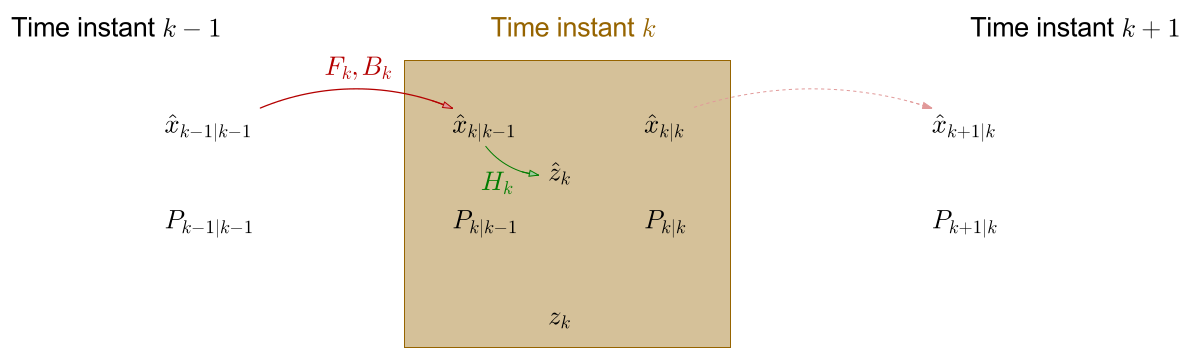
\includegraphics[scale=0.5]{images/kfb}
\caption{Representaci\'on del proceso de predicci\'on (obtenci\'on de cantidades a priori) de las cantidades $\hat{x}_{k|k-1}$ y $P_{k|k-1}$;  y de correcci\'on (estimaci\'on a posteriori) para obtener las cantidades $\hat{x}_{k|k}$ y $P_{k|k}$. Para el siguiente paso, $k+1$, estas estimaciones pasan a ser entrada (\textit{input}) de un nuevo proceso de predicci\'on: $\hat{x}_{k+1|k}$ y $P_{k+1|k}$. \textit{E. Matsinos, 2016. The Kalman Filter: a didactical overview.}}
\label{fig:kfb}
\end{figure}
\subsubsection{Ejemplo: Part\'icula acelerada externamente}
Consideremos un veh\'iculo sobre un riel sin curvas y sin fricci\'on, de tal forma que se pueda asumir un movimiento unidimensional. Inicialmente el veh\'iculo se encontrar\'a en una posici\'on definida como $x_0=0$ y en reposo, $\dot{x}_0=0$, cuando s\'ubitamente es perturbado por fuerzas externas que lo inducen a moverse. Entonces, para monitorear su movimiento se hace un muestreo cada $\Delta t$ segundos. Sin embargo estas mediciones no son del todo precisas, por lo que podr\'ia desearse determinar la posici\'on y velocidad del objeto en cada instante a trav\'es de un modelo.
\bigskip

En esta oportunidad, el vector de estado va a estar dado por:

\begin{align}
x_k &= \begin{bmatrix}
x\\ \dot{x}
\end{bmatrix},
\label{eq:example_state} 
\end{align} 
donde $x$ representa la posici\'on del m\'ovil y $\dot{x}$ su velocidad.
\bigskip

Si asumimos que entre los instantes $k-1$ y $k$, estas fuerzas externas causan una aceleraci\'on constante, $a_k$, cuya distribuci\'on es una normal de media 0 y desviaci\'on est\'andar $\sigma_a$, podemos aplicar las leyes f\'isicas de movimiento, se tiene

\begin{equation}
x_{k} = F_k x_{k-1} + G_k a_k,
\label{eq:example_pred_orig} 
\end{equation}

con 

\begin{align}
F_k &= \begin{bmatrix}
1 & \Delta t\\
0 & 1 
\end{bmatrix},
\label{eq:example_F}
\end{align}


mientras que $G_k$ agrega la componente de aceleraci\'on sobre el sistema:

\begin{align}
G_k &= \begin{bmatrix}
\frac{1}{2} \Delta t^2\\
\Delta t
\end{bmatrix}.
\label{eq:example_G}
\end{align}

De la Ecuaci\'on \ref{eq:example_pred_orig} se desprende que el t\'ermino original $B_k u_k$ ha sido reemplazado por $G_k a_k$; esto se debe a que la \'ultima cantidad corresponde a perturbaciones externas, y no existen entradas de control (perturbaciones controladas o conocidas, por ejemplo, que el riel posea fricci\'on). De esto \'ultimo se deduce que $q_k = G_k a_k$.
\bigskip

De la expresi\'on \ref{eq:example_G} es posible calcular $Q_k$: 

\begin{align}
Q_k = G_k G_k^T \sigma_a^2 &= \begin{bmatrix}
\frac{1}{4}\Delta t^4 & \frac{1}{2}\Delta t^3\\
 \frac{1}{2}\Delta t^3 & \Delta t^2
\end{bmatrix} \sigma_a^2. 
\end{align}

En cada paso temporal $\Delta t$ se realiza una medici\'on, la cual incluye ruido, de la posici\'on del veh\'iculo. Sea $r_k$ el ruido de la medici\'on:

\begin{equation}
z_k = H_k x_k + r_k,
\label{eq:corr_example}
\end{equation}

en donde, $H_k = \begin{bmatrix}
1 & 0
\end{bmatrix}$, y desde la cantidad $r_k$ se calcula $R_k$: $R_k = E[v_kv_k^T]=[\sigma_{z}^2]$.

Con este sistema, podemos modelar el filtro y usar las siguientes condiciones iniciales:

\begin{align}
\hat{x}_{0|0} &= \begin{bmatrix}
0\\
0
\end{bmatrix},
\label{eq:init_state} 
\end{align} 

\begin{align}
P_{0|0} &= \begin{bmatrix}
\sigma_{x}^2 & 0\\
0 & \sigma_{\dot{x}}^2
\end{bmatrix}.
\label{eq:init_cov} 
\end{align} 

En donde la Ecuaci\'on \ref{eq:init_state} describe el estado inicial del sistema y \ref{eq:init_cov} la matriz de covarianza inicial, la cual, dependiendo de si se conoce perfectamente la posici\'on del objeto, todos sus valores ser\'an cero; de no conocerse bien la posici\'on del m\'ovil, entonces los valores de $\sigma_{x}$ y $\sigma_{\dot{x}}$ deber\'an considerarse mayores a cero.
\bigskip

Este modelo fue el elegido para estimar la evoluci\'on del flujo y su velocidad en la implementaci\'on de la versi\'on b\'asica del filtro en el programa original (y por consiguiente, en su \textit{refactoring}).
%\begin{equation}
%x_{k|k-1} = F_k x_{k-1|k-1} + G_k a_k
%\label{eq:example_pred} 
%\end{equation}



\subsection{Filtro de Kalman de M\'axima Correntrop\'ia}

El filtro de Kalman basado en m\'axima correntrop\'ia \cite{badong}, difiere del filtro de Kalman tradicional (b\'asico) en que no asume gaussianidad en las observaciones, considerando casos en que una se\~nal puede ser perturbada por pulsos de ruido que sigan una distribuci\'on de cola pesada. En esta oportunidad se utiliza el \textit{criterio de m\'axima correntrop\'ia} del error para el proceso de correcci\'on. 
\bigskip

La correntrop\'ia es una medida de similitud entre dos variables aleatorias. Supongamos, $X,Z \in \mathbb{R}$ con una distribuci\'on conjunta $F_{XZ} (x,z)$. Definimos la correntrop\'ia matem\'aticamente como:

\begin{equation}
V(X,Z) = E[\kappa(X,Z)] = \int \kappa(x,z) dF_{XZ} (x,z),
\label{eq:eqcorr}
\end{equation}
\noindent
donde $E$ representa al operador de esperanza y $\kappa(\cdot,\cdot)$ corresponde a un \gls{kernel} Mercer invariante a desplazamientos (teorema de Mercer \cite{mercer}). Para este filtro se emplea una funci\'on de kernel Gaussiana (que satisface la condici\'on de Mercer), dado por

\begin{equation}
\kappa(x, z) = G_{\sigma} (e) = exp \left(-\dfrac{e^2}{2\sigma^2} \right),
\label{eq:eqkappa}
\end{equation}

donde $e=x-z$ es el error.
\bigskip

Usualmente, en situaciones pr\'acticas, s\'olo se dispone de una cantidad limitada de datos y la distribuci\'on conjunta $F_{XZ}$ podr\'ia ser desconocida, por lo que es posible estimar la correntrop\'ia usando un estimador del promedio sobre la muestra:

\begin{equation}
\hat{V}(X,Z) = \dfrac{1}{M} \sum_{i=1}^M G_{\sigma} (e_i),
\label{eq:eqcoor_est}
\end{equation} 

en que $e_i = x_i - z_i$, con $\{x_i,z_i\}_{i=1}^M$ siendo $M$ el n\'umero de muestras extra\'idas de $F_{XZ}$~\cite{badong}.
\bigskip

Considerando un sistema lineal, descrito por las ecuaciones de estado (\ref{eq:mcc01}) y correci\'on (\ref{eq:mcc02}) 

\begin{equation}
x_{k} = F_{k-1}x_{k-1} + q_{k-1}
\label{eq:mcc01}
\end{equation}
\begin{equation}
\hat{z}_k = H_k x_{k} + r_k.
\label{eq:mcc02}
\end{equation}

Donde $F_{k-1}$ y $H_{k-1}$ corresponden a la matriz de transici\'on de estado y matriz de observaci\'on respectivamente; y los t\'erminos $q_{k-1}$ y $r_k$ corresponden a los vectores de ruido del proceso y de medici\'on, respectivamente, de media cero y matrices de covarianza:
\bigskip

\begin{equation}
\begin{gathered}
E[q_{k-1}q_{k-1}^T] = Q_{k-1}, \\
E[r_{k}r_{k}^T] = R_{k}
\end{gathered}
\end{equation}

Usando la media (donde $\hat{q}_k=0$) y la matriz de covarianza prior, el proceso de predicci\'on queda como: 

\begin{equation}
\begin{gathered}
\hat{x}_{k|k-1} = F_{k-1}\hat{x}_{k-1|k-1},\\
P_{k|k-1} = F_{k-1}P_{k-1|k-1}F_{k-1}^T + Q_{k-1}.
\end{gathered}
\label{eq:mean_pred}
\end{equation}


Luego, la correcci\'on comienza con el c\'alculo de la ganancia de Kalman:

\begin{equation}
K_k = P_{k|k-1} H_k^T (H_kP_{k|k-1}H_k^T + R_k)^{-1},
\label{eq:mcc_kalman_gain}
\end{equation}

y contin\'ua con la determinaci\'on del estado y matriz de covarianza posterior:

\begin{equation}
\hat{x}_{k|k} = \hat{x}_{k|k-1} + K_k(z_k - H_k \hat{x}_{k|k-1}),
\label{eq:mcc_post_state}
\end{equation}

\begin{equation}
P_{k|k} = (I - K_kH_k)P_{k|k-1} (I - K_kH_k)^T + K_kR_kK_k^T
\label{eq:mcc_post_cov}
\end{equation}

donde $I$ corresponde a la matriz identidad (Ecuaci\'on \ref{eq:mcc_post_cov}).
\bigskip

El modelo lineal descrito en las Ecuaciones \ref{eq:mcc01} y \ref{eq:mcc02} pueden reescribirse usando la media prior (\ref{eq:mean_pred}), obteni\'endose:


  \begin{align}
    \begin{bmatrix}
    \hat{x}_{k|k-1}\\
    y_k
	\end{bmatrix}     &= \begin{bmatrix}
          I \\
           H_{k}
         \end{bmatrix} x_k + \nu_k
         \label{eq:nu_det01}
  \end{align} 

\begin{align}
\nu_k &= \begin{bmatrix}
-(x_k - \hat{x}_{k|k-1})\\
r_k
\end{bmatrix} .
\label{eq:nu_det02}
\end{align}

De aqu\'i se desprende, usando las expresiones prior (\ref{eq:mean_pred}), el valor esperado:

\begin{align}
E \lbrack \nu_k \nu_k^T \rbrack &= \begin{bmatrix}
P_{k|k-1} & 0 \\
0 & R_k
\end{bmatrix}\\
&= \begin{bmatrix}
B_{k|k-1; P}B_{k|k-1; P}^T & 0\\
0 &  B_{k|k-1; R}B_{k|k-1; R}^T
\end{bmatrix}\\
& = B_kB_k^T,
\end{align}

donde $B_k$ puede ser obtenido a partir de la descomposici\'on de Cholesky del t\'ermino $E \lbrack \nu_k \nu_k^T \rbrack$ (las cantidades $B_{k|k-1; P}$ y $B_{k|k-1; R}$ corresponden a los valores asociados a la covarianza del estado estimado y del ruido de la medici\'on, $R_k$, respectivamente).
\bigskip

Multiplicando la ecuaci\'on \ref{eq:nu_det01} por la izquierda por $B_k^{-1}$, se obtiene:

\begin{equation}
D_k = W_k x_k + e_k,
\label{eq:D}
\end{equation}

donde $D_k = B^{-1}_k \begin{bmatrix}
\hat{x}_{k|k-1}\\ y_k
\end{bmatrix}$, $W_k = B^{-1}_k \begin{bmatrix}
I\\ H_k
\end{bmatrix}$, $e_k = B^{-1}_k \nu_k$.  
\bigskip

Proponiendo una \textit{funci\'on de costo} basada en la funci\'on de m\'axima correntrop\'ia (ver Ecuaci\'on de correntrop\'ia, \ref{eq:eqcoor_est}):

\begin{equation}
J_{L}(x_k) = \dfrac{1}{L} \sum_{i=1}^L G_{\sigma} (d_{i,k} - w_{i,k}x_k),
\label{eq:costo}
\end{equation}

donde $d_{i, k}$ corresponde al i-\'esimo elemento del vector $D_k$, $w_{i,k}$ es la i-\'esima fila de la matriz $W_k$ y $L$ es la suma de las dimensiones de los vectores de estado ($x_k$), $N$  y medici\'on ($y_k$), $N'$; es decir $L=N+N'$.

Luego, bajo el criterio de m\'axima correntrop\'ia, se tiene que para el estado \'optimo de $x_k$, $\hat{x}_k$

\begin{equation}
\hat{x}_k = \argmax_{x_k} J_{L}(x_k)= \argmax_{x_k} (\sum_{i=1}^L G_{\sigma} (e_{i,k})),
\label{eq:max}
\end{equation}
\bigskip

en que $e_{i,k}$ es el i-\'esimo elemento de $e_k$:

\begin{equation}
e_{i,k}= d_{i, k} - w_{i,k}x_k.
\label{eq:ei}
\end{equation}

Por tanto, la soluci\'on \'optima puede obtenerse resolviendo:

\begin{equation}
\dfrac{\partial J_L(x_k)}{\partial x_k} = \sum_{i=1}^L \lbrack G_{\sigma}(e_{i,k}) w_{i, k}^T (d_{i,k} -w_{i,k}x_k)  \rbrack =0, 
\label{eq:optimal}
\end{equation}
\bigskip

desde donde se tiene:

\begin{equation}
x_k = \lbrace \sum_{i=1}^L \lbrack G_{\sigma} (e_{i,k}) w_{i,k}^T w_{i,k} \rbrack \rbrace^{-1} \times
\lbrace \sum_{i=1}^L \lbrack G_{\sigma} (e_{i,k}) w_{i,k}^T d_{i,k} \rbrack \rbrace
\label{eq:optima1}
\end{equation}

La Ecuaci\'on \ref{eq:optima1} corresponde realmente a una ecuaci\'on de \textit{punto fijo} de $x_k$ (por \ref{eq:ei}) y puede ser reescrita como:

\begin{equation}
x_k = f(x_k) = \left( \sum_{i=1}^{L} \lbrack G_{\sigma} (d_{i,k} - w_{i,k}x_k) w_{i,k}^T w_{i,k}  \rbrack \right)^-1 \times \left( \sum_{i=1}^{L} \lbrack G_{\sigma} (d_{i,k} - w_{i,k}x_k) w_{i,k}^T d_{i,k}  \rbrack \right).
\label{eq:optimal2}
\end{equation}
\bigskip

Un algoritmo iterativo de punto fijo puede ser obtenido usando $\hat{x}_{k, t+1} = f(\hat{x}_{k, t})$, en donde $\hat{x}_{k, t}$ denota la soluci\'on en un punto fijo en la iteraci\'on $t$ (en el instante $k$).
\bigskip

La Ecuaci\'on \ref{eq:optima1} entonces puede ser expresada como:
\begin{equation}
x_k = \left( W^T_k C_k W_k \right)^{-1} W^T_k C_k D_k
\end{equation}

en que $C_k = \begin{bmatrix}
C^{x}_k & 0\\
0 & C^{z}_k
\end{bmatrix} $, con 

\begin{equation}
C^{x}_{k}= diag(G_{\sigma}(e_{1, k}),..., G_{\sigma}(e_{N, k})),
\label{eq:Cx}
\end{equation}

\begin{equation}
{C^{z}_{k}}= diag(G_{\sigma}(e_{N+1, k}),..., G_{\sigma}(e_{N+N', k})).
\label{eq:Cz}
\end{equation}

Con estas derivaciones es posible resumir el algoritmo de estimaci\'on por filtro de Kalman de m\'axima correntrop\'ia como sigue \cite{badong}:

\begin{enumerate}
\item Escoger un $\sigma$ para el ancho del kernel apropiado, y un $\epsilon$ cuyo valor sea $0 < \epsilon < 1$ (lo suficientemente peque\~no para obtener una buena convergencia). Definir un estado estimado inicial $\hat{x}_{0|0}$ y una matriz de covarianza inicial $P_{0|0}$. Definir $k=1$.
\item Usar las Ecuaciones \ref{eq:mean_pred} para obtener $\hat{x}_{k|k-1}$ y $P_{k|k-1}$, y usar descomposici\'on de Cholesky para obtener $B_{k|k-1;P}$.
\item Definir $t=1$ y $\hat{x}_{k|k,0} = \hat{x}_{k|k-1}$, donde $\hat{x}_{k|k,t}$ denota el estado estimado en la iteraci\'on $t$ del algoritmo de punto fijo.
\item Usar los siguientes pasos para calcular $\hat{x}_{k|k}$:

\begin{equation}
\hat{x}_{k|k,t} = \hat{x}_{k|k-1,t} + \tilde{K}_k (z_k - H_k \hat{x}_{k|k-1}),
\end{equation}
con 

\begin{equation}
\tilde{K} = \tilde{P}_{k|k-1} H_k^T (H_k \tilde{P}_{k|k-1} H_k^T + \tilde{R}_k)^{-1}, 
\label{eq:eq14}
\end{equation}

\begin{equation}
\tilde{P}_{k|k-1} = B_{p, k|k-1} \tilde{C}_{x, k}^{-1}B_{p, k|k-1}^T,
\label{eq:eq13}
\end{equation}

\begin{equation}
\tilde{R}_k = B_{r, k} \tilde{C}_{y, k}^{-1}B_{r, k|k-1}^T,
\label{eq:eq12}
\end{equation}

\begin{equation}
\tilde{C^{x}_{k}}= diag(G_{\sigma}(\tilde{e}_{1, k}),..., G_{\sigma}(\tilde{e}_{N, k})),
\label{eq:eq10}
\end{equation}

\begin{equation}
\tilde{C^{z}_{k}}= diag(G_{\sigma}(\tilde{e}_{N+1, k}),..., G_{\sigma}(\tilde{e}_{N+N', k})).
\label{eq:eq11}
\end{equation}


\begin{equation}
\tilde{e}_{i,k} = d_{i,k} - w_{i,k} \hat{x}_{t-1, k|k}.
\label{eq:eq9}
\end{equation}

\item Posteriormente se compara la estimaci\'on de la iteraci\'on actual con la estimaci\'on de la \'ultima:
\begin{equation}
\dfrac{\parallel  \hat{x}_{t, k|k} - \hat{x}_{t-1, k|k} \parallel }{\parallel \hat{x}_{t-1, k|k} \parallel} \leq \epsilon.
\label{eq:eq16}
\end{equation}

Si se cumple la relaci\'on de la Ecuaci\'on \ref{eq:eq16}, entonces $\hat{x}_{k|k} = \hat{x}_{k|k,t}$, y se contin\'ua con el siguiente paso; en caso contrario $t\rightarrow t+1$, y se vuelve al paso (4).

\item Finalmente, se actualiza la matriz de covarianza posterior con 
\begin{equation}
P_{k|k} = \left(I - \tilde{K}_kH_k \right)P_{k|k-1} \left(I - \tilde{K}_k H_k \right)^T + \tilde{K}_kR_k\tilde{K}^T_k,
\label{eq:eq17}
\end{equation}
continuando con el instante $k+1$ en el paso (2).
\end{enumerate}


\subsection{Filtro de Kalman Unscented (UKF)}
\label{ssec:ukf}
Este filtro corresponde a aquel que se pretende agregar a la familia de filtros ya desarrollada en el programa base.
\bigskip

\begin{enumerate}
\item \textbf{Fase predictiva:}\\
En esta versi\'on del filtro \cite{ukf} ya no se habla de matrices de transici\'on de estado, $F_k$, ni de matrices de transformaci\'on de estado-a-medici\'on, $H_k$, sino m\'as bien de funciones diferenciables $f$ y $h$ respectivamente, para describir la transici\'on de estados  y la transformaci\'on de estos a estimaciones a priori. Sin embargo, previo a estas transiciones se deben seleccionar 2N+1 puntos representativos alrededor de $\hat{x}_{k-1|k-1}$ y evaluar estos en la funci\'on no lineal $f$, para obtener las estimaciones de $\hat{x}_{k|k-1}$ y $P_{k|k-1}$. Estos puntos se conocen como \textit{puntos sigma}. En la Figura \ref{fig:fukf} se visualiza el proceso de predicci\'on al momento de obtener el primer conjunto de \textit{puntos sigma}, propagarlos usando la funci\'on $f$ y obtener $\hat{x}_{k|k-1}$ y $P_{k|k-1}$, es decir, la matriz de estados y de covarianza \textit{a priori}. 

\begin{figure}[h!]
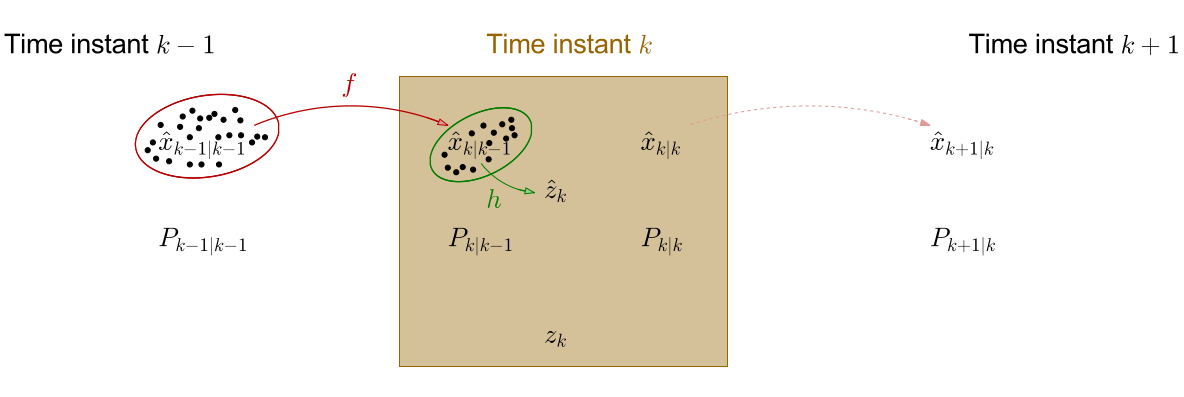
\includegraphics[scale=.5]{images/ukf}
\caption{Representaci\'on del funcionamiento del filtro UKF. En esta oportunidad se hace uso de la funci\'on $f$ y $h$ para obtener la predicci\'on y la correcci\'on. Esto se logra con la evaluaci\'on de los 2N+1 \textit{puntos sigma} generados durante la etapa de predicci\'on (y posteriormente en la etapa de correcci\'on). \textit{E. Matsinos, 2016. The Kalman Filter: a didactical overview.}}
\label{fig:fukf} 
\end{figure}

La generaci\'on de los 2N+1 puntos, se realiza a partir de la \'ultima estimaci\'on $\hat{x}_{k-1|k-1}$  de la siguiente forma:
\begin{equation}
\label{eq:eq18}
\begin{gathered}
\bar{x}_{k-1| k-1}^0 = \hat{x}_{k-1|k-1}\\
\bar{x}_{k-1| k-1}^0 = \hat{x}_{k-1|k-1}+ \chi_i, \quad  \forall i \in [1, N]\\
\bar{x}_{k-1| k-1}^0 = \hat{x}_{k-1|k-1}- \chi_{i-N}, \quad  \forall i \in [N+1, 2N],
\end{gathered}
\end{equation}
donde la cantidad $\chi_i$ corresponde a la i-\'esima columna de la \textit{ra\'iz cuadrada} de la matriz:

 \begin{equation}
 (N+\lambda) P_{k-1 | k-1}.
 \label{eq:eq19}
 \end{equation}
La matriz (\ref{eq:eq19}) puede obtenerse a partir de la descomposic\'on de Cholesky. Por otro lado los puntos sigma se generan junto a dos conjuntos de pesos: $\lbrace w_x^{i} \rbrace$ y $\lbrace w_p^{i} \rbrace$. El primer conjunto se emplea en la estimaci\'on del estado y la predicci\'on del estado, mientras que el segundo conjunto es usado para obtener las matrices de covarianza. Estos pesos son definidos como:
\begin{equation}
\label{eq:eq20}
\begin{gathered}
w^0_x = \dfrac{\lambda}{N+\lambda}\\
w^0_p = w^0_x + 1 - \alpha^2 + \beta\\
w^i_x = w^i_p = \dfrac{1}{2(N+\lambda)}\\
\sum_i^{2N} w^i_x = 1.
\end{gathered}
\end{equation}
De la Ecuaci\'on \ref{eq:eq20} se desprende que los pesos $w_x^i$ son normalizados. Por otro lado, el par\'ametro $\lambda$ se puede escribir en t\'erminos de los valores de $\alpha \in \left( 0,1\right]$ y $\kappa$ seg\'un la expresi\'on siguiente:%\ref{eq:eq21}

\begin{equation}
\label{eq:eq21}
\lambda = \alpha^2  (N + \kappa)- N.
\end{equation}

Los par\'ametros $\alpha$, $\beta$ y $\kappa$ deben ser ajustados acorde al problema que se est\'a estudiando.
\bigskip

Con esto, es posible escribir las ecuaciones de la fase predictiva.
\begin{itemize}
\item Estimaci\'on a priori de los estados. La ecuaci\'on correspondiente es:\\
\begin{equation}
\label{eq:eq22}
\hat{x}_{k|k-1} = \sum_{i=0}^{2N} w_{x}^i f(\bar{x}^i_{k-1|k-1}).
\end{equation}

\item Estimaci\'on a priori de la matriz de covarianza. La ecuaci\'on correspondiente es:\\

\begin{equation}
\label{eq:eq23}
P_{k|k-1} = \sum_{i=0}^{2N} w_p^i \left( f(\bar{x}^i_{k-1|k-1})  - \hat{x}_{k|k-1}\right)\left( f(\bar{x}^i_{k-1|k-1}) - \hat{x}_{k|k-1}  \right)^T + Q_k.
\end{equation}
\end{itemize}


\item \textbf{Fase correctiva:}\\
Durante la fase de correcci\'on, nuevamente se seleccionan 2N+1 puntos representativos, alrededor de $\hat{x}_{k|k-1}$. Estos posteriormente son evaluados en la funci\'on no-lineal $h$.

\begin{equation}
\label{eq:eq24}
\begin{gathered}
\bar{y}_{k-1| k-1}^0 = \hat{x}_{k|k-1}\\
\bar{y}_{k-1| k-1}^i = \hat{x}_{k|k-1}+ \psi_i, \quad  \forall i \in [1, N]\\
\bar{y}_{k-1| k-1}^i = \hat{x}_{k|k-1}- \psi_{i-N}, \quad  \forall i \in [N+1, 2N].\\
\end{gathered}
\end{equation}
La cantidad $\psi_i$ representa la i-\'esima columna de la matriz de \textit{ra\'iz cuadrada} $(N+\lambda)P_{k|k-1}$.

Las ecuaciones del proceso de correcci\'on, por tanto, quedan como sigue:
\begin{itemize}
\item Predicci\'on de las medidas:\\
\begin{equation}
\label{eq:eq25}
\hat{z}_{k} = \sum_{i=0}^{2N} w_x^i h(y_{k|k-1}^{-i}).
\end{equation}
\item Los residuos de las mediciones pueden obtenerse como:\\
\begin{equation}
\tilde{z}_k = z_k - \hat{z}_k.
\label{eq:eq26}
\end{equation}
\item La matriz de innovaci\'on:\\
\begin{equation}
S_k = \sum_{i=0}^{2N} w_p^i (h(y_{k|k-1}^{-i}) - \hat{z}_k)(h(y_{k|k-1}^{-i})^T + R_k.
\label{eq:eq27}
\end{equation}
\item La matriz de covarianza cruzada de estado a medida se describe como:\\
\begin{equation}
C_k = \sum_{i=0}^{2N} w_p^i ( f(\bar{x}^i_{k-1 | k-1})- \hat{x}_{k|k-1} )( h(y_{k|k-1}^{-i}) - \hat{z}_k )^T.
\label{eq:eq28}
\end{equation}
\item La ganancia \'optima finalmente queda:\\
\begin{equation}
K_k = C_kS_k^{-1}.
\label{eq:eq29}
\end{equation}
\item La estimaci\'on \textit{a posteriori} de estado:\\
\begin{equation}
\label{eq:eq30}
 \hat{x}_{k|k} =  \hat{x}_{k|k-1} + K_k \tilde{z}.
\end{equation}
\item Por otro lado, la ecuaci\'on para la matriz de covarianza:\\
\begin{equation}
\label{eq:eq31}
P_{k|k} = P_{k|k-1} - K_kS_kK_k^T.
\end{equation}
\end{itemize}
Los pesos $w_x^i$ y $w_p^i$ son los mismos calculados en la expresi\'on \ref{eq:eq20}, de la fase de predicci\'on.
\end{enumerate}
\bigskip

\subsubsection{Nota}
En este trabajo se considerar\'a un modelo no lineal sobre el paso del tiempo medido desde la primera observaci\'on realizada por el survey: $t_0$. Es decir, la no linealidad no se aplicar\'a sobre la estimaci\'on realizada sobre el paso anterior.

\begin{align}
\begin{bmatrix}
x_k(\Delta t)\\
\dot{x}_k(\Delta t)
\end{bmatrix}  &= \begin{bmatrix}
x_{k-1}\\
0
\end{bmatrix} + \sigma_a\begin{bmatrix}
\Delta t ^{r}\\
\frac{1}{r}\Delta t^{r-1}
\end{bmatrix} = f(x_{k-1}, \Delta t)
\label{eq:modelunscented}
\end{align}

Para la implementaci\'on de este filtro, se usar\'a el modelo descrito en la ecuaci\'on \ref{eq:modelunscented}. El valor de $\sigma_a$ corresponde a un t\'ermino similar al de una aceleraci\'on (como el modelo usado para el filtro b\'asico), para conservar las unidades de posici\'on y velocidad.

\section{Laboratorio Nacional de Computaci\'on de Alto Desempe\~no (NLHPC)}
El National Laboratory for High Performance Computing (NLHPC) es un proyecto asociativo, financiado por el PIA de CONICYT el cual dispone de un potente sistema computacional que est\'a disponible a la comunidad cient\'ifica y acad\'emica nacional (instituciones de investigaci\'on, industria y universidades), estimulando su uso en el desarrollo de \'areas de investigaci\'on que requieran de herramientas computacionales robustas que deban ser usadas de manera intensiva. 
\bigskip

El supercomputador del NLHPC disponible para la comunidad investigadora desde el 2014 en las instalaciones del Centro de Modelamiento Matem\'atico (CMM) de la Universidad de Chile.  

\begin{itemize}
\item 132 nodos de c\'omputo HP (128 nodos HP SL230 y 4 nodos HP SL250), cada uno con dos procesadores de 10 cores Intel Xeon Ivy Bridge E5-2660 V2.
\item 2640 n\'ucleos
\item 6.25 TB de RAM
\item 274TB de almacenamiento Lustre (DDN EXAScaler)
\item 12 co-procesadores Intel Xeon Phi5110p de 2 TFlops
\item Capacidad de c\'omputo de 70 TFlops 
\end{itemize} 

Para la realizaci\'on de este trabajo de t\'itulo se hizo uso de uno de los nodos del cl\'uster de Leftraru, y en la ejecuci\'on de las pruebas se emplearon cuatro cores, 2400 MB por cada CPU (m\'axima RAM permitida) y un \textit{job-array} de largo 93.

